
\documentclass[conference]{IEEEtran}
\IEEEoverridecommandlockouts
% The preceding line is only needed to identify funding in the first footnote. If that is unneeded, please comment it out.
\usepackage{cite}
\usepackage{amsmath,amssymb,amsfonts}
\usepackage{algorithmic}
\usepackage{graphicx}
\usepackage{textcomp}
\usepackage{xcolor}
\usepackage[spanish]{babel} 
\def\BibTeX{{\rm B\kern-.05em{\sc i\kern-.025em b}\kern-.08em
    T\kern-.1667em\lower.7ex\hbox{E}\kern-.125emX}}



\begin{document}

\title{La importancia de las habilidades blandas en trabajos de ciencia y tecnología. Cómo fomentarlas desde el ámbito académico
}

\author{\IEEEauthorblockN{Juan Cristian Miguel}
\IEEEauthorblockA{\textit{Modelos de Organizaciones y Sistemas de Información} \\
\textit{Especialización en Ingeniería de Sistemas de Información (UTN FRBA)}\\
Buenos Aires, Argentina \\
juancristianmiguel@gmail.com}
}

\maketitle

% This file type can be used to insert custom commands, preamble settings, or whatever material should be printed directly rather than treated as part of the structure of the work.

\begin{abstract}
La falta de profesionales que dispongan de un buen repertorio de habilidades blandas no es un problema reciente. La tecnología avanza a un paso agigantado. Desde hace años la dinámica laboral demanda soluciones novedosas que involucran saberes diversos, pero actualmente los conocimientos técnicos no son suficientes. Las habilidades de comunicación, gestión de proyectos, auto-presentación y muchas más son cada vez más necesarias en algunos contextos. Estas cualidades están ligadas a experiencias y características personales, propias de cada persona, lo que torna a su aprendizaje y enseñanza todo un desafío. En el presente artículo se expone un análisis de esta problemática y se otorgan propuestas para fomentarlas en enseñanza universitaria, técnica y científica, principalmente ingeniería y carreras afines.
\end{abstract}

\begin{IEEEkeywords}
	soft skills, habilidades blandas, employability, métodos de enseñanza, universidad, ingeniería
\end{IEEEkeywords}

\section{Introducción}
\label{scrivauto:1}

La dinámica laboral en materias de ciencia y tecnología ha experimentado cambios a lo largo del tiempo a causa de diversos factores. Las necesidades actuales son muy diferentes respecto a años atrás y los proyectos requieren saberes de múltiples áreas técnicas. En este contexto, es lógico suponer que se necesitan profesionales y equipos interdisciplinarios que sean capaces de atender los requerimientos del mercado y la industria. No obstante, no es tan simple visualizar que los conocimientos técnicos, adquiridos en instituciones académicas y carreras de grado de todo tipo, no son suficientes para acometer esta tarea; las habilidades blandas (en ocasiones referenciadas como ``no técnicas``) también son necesarias. 
Hoy en día, los empleadores en puestos de trabajos buscan cada día más profesionales que dispongan de ciertas habilidades blandas. Estudios recientes por el contrario demostraron que los graduados en universidades poseen una carencia de ellas \cite{b1}.
En este escenario, surgen las siguientes preguntas:

\begin{itemize}
    \item ¿Qué son exactamente las habilidades blandas y por qué son necesarias?
    \item ¿Existen formas de promoverlas o enseñarlas desde el ámbito académico?
\end{itemize}

El propósito de este artículo es dar una respuesta a ambos interrogantes.

\section{Pertinencia con el seminario}
\label{scrivauto:2}

Uno de los temas a tratar en este seminario es la gestión del conocimiento. Según Hubert Saint-Onge, la misma se define como ``la habilidad de desarrollar, mantener, influenciar y renovar los activos intangibles llamados Capital de Conocimiento o Capital Intelectual``. En este sentido, se puede entender la promoción de habilidades blandas como el desarrollo de un conjunto de activos intangibles de carácter no técnico, necesarios para encarar los proyectos multidisciplinarios la industria actual.
Otro punto de pertinencia radica en el hecho de que el seminario motiva el ejercer una mirada crítica de la tecnología en términos de impacto social. Esta iniciativa está estrechamente ligada con habilidades blandas como ser la ética laboral, la empatía, nociones de preservación del medio ambiente y otras similares de gran implicancia social e interpersonal.

\section{Definición de habilidades blandas}
\label{scrivauto:3}

Antes de comenzar con el análisis propuesto para este documento, es conveniente hallar una definición sobre qué son las habilidades blandas, en contraposición con las habilidades duras. Esto brindará un contexto base para profundizar en las cuestiones particulares de la problemática expuesta.

Las habilidades duras son un tipo de conocimiento que puede documentarse y crearse fácilmente, escribirse y transferirse por medio de instituciones educativas mediante mecanismos conductivos e incorporación de cultura \cite{b5}. Generalmente se basan en el contexto específico en que se utilizan y suelen interpretarse como aquellos procedimientos administrativas  o técnicos que pueden ser medidos y cuantificados \cite{b4}. 

Las habilidades duras, además, están vinculadas a comportamientos explícitos, es decir, pueden producir algo visible y concreto que es susceptible de ser puesto a prueba mediante métodos técnicos y prácticos \cite{b5}.

En cuanto a las habilidades blandas, obtener una única definición es una tarea compleja. Algunos autores opinan que son saberes que permanecen en la mente humana, por ende son difíciles de formular y caracterizar. Están íntimamente relacionadas con nuestras acciones y experiencias, incluyendo los ideales personales, valores y emociones \cite{b5}.  Perreault, por su parte, en el año 2004 las definió como habilidades y características especiales que permiten diferenciar personas que tienen un crecimiento profesional y experiencia similares \cite{b4}. En ocasiones, algunos autores también las interpretan como habilidades ``no técnicas`` \cite{b3} en contraposición a las habilidades duras. Sin embargo, esta definición no es determinante ni satisfactoria. Citando la Real Academia Española (RAE), la técnica no es sino un ``conjunto de procedimientos y recursos de que se sirve una ciencia o un arte``. En este sentido, habilidades blandas como la gestión del tiempo, en pos de aumentar la productividad laboral, requieren de técnicas mínimas de fácil aprendizaje, en conjunto con las experiencias e ideas personales de cada individuo. Las habilidades blandas, entonces, se complementan con las habilidades duras.

En base a todo lo antedicho, se concluye que las habilidades blandas son un conjunto de actitudes personales e intransferibles, motivadas por nuestras experiencias vividas y nuestra personalidad particular. Debido a esto, no es posible adquirir esta clase de habilidades por los mismos medios con los que se adquieren los conocimientos técnicos, sino que se requieren actividades y procedimientos diferentes que incentiven a que cada estudiante experimente y las desarrolle por su cuenta. Por lo tanto, mientras que una institución educativa, sea del nivel que sea, es suficientemente capaz inculcar los conocimientos técnicos de una ciencia en concreto, cada individuo sólo se nutre de ciertas experiencias en ellas.

% Acá me falta explicar cositas




\section{Primera clasificación posible de habilidades blandas}
\label{scrivauto:4}

Como ya hemos introducido, las habilidades blandas están determinadas por aspectos o cualidades características de una persona, íntimamente relacionadas a sus experiencias, sus valores y sus emociones. Pero a menudo una persona interactúa con otras, se comunica y toma decisiones basadas en un conjunto de creencias y argumentos. Debido a esto, es factible suponer que hay distintos tipos de estas habilidades: algunas netamente individuales; otras, en cambio, interpersonales.

Si bien no hay un consenso total acerca de cómo clasificarlas, desde un punto de vista psicológico se pueden dividir en cuatro categorías: ``Necesidades y razones, ``Relacionadas a valores``, ``Comportamentales`` y ``Emocionales`` \cite{b7}. La figura \ref{fig:tipos_soft_skills} ilustra estos cuatro grupos y algunos ejemplos.



\begin{figure}[htbp]
\centering
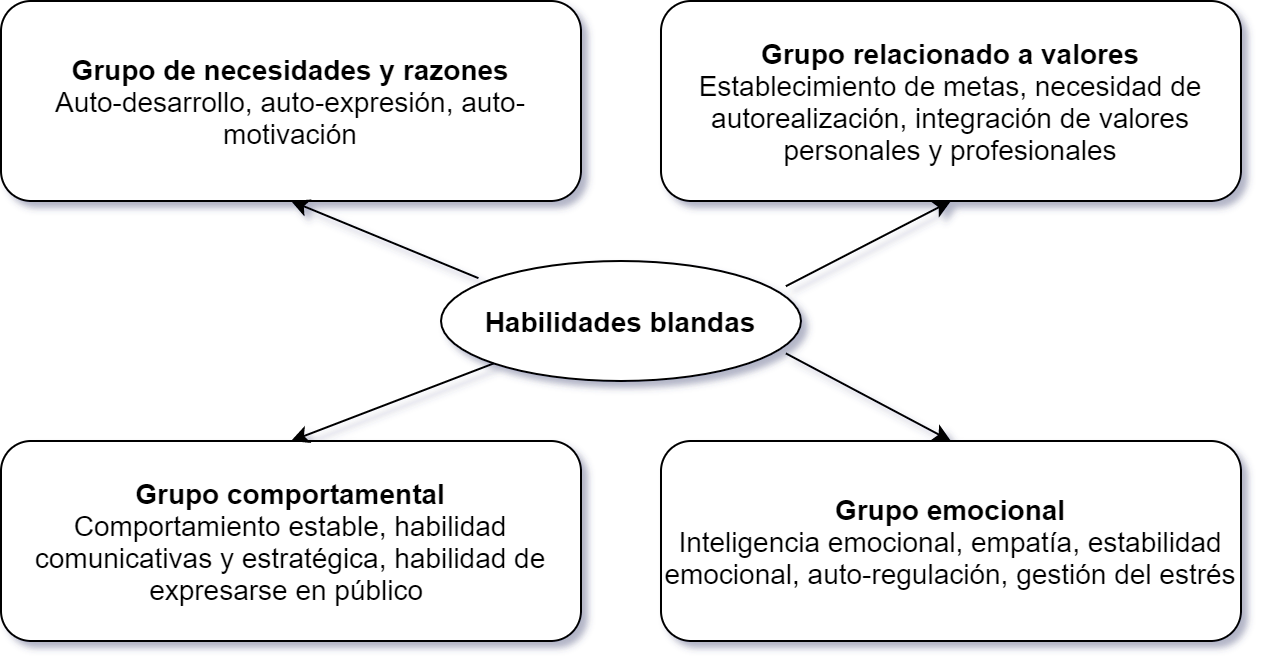
\includegraphics[width=250pt,height=131pt]{Grupos_Soft_skills.png}

\caption{Clafisicación de habilidades blandas en función de cuatro aspectos constitutivos \cite{b7}}
\label{fig:tipos_soft_skills}
\end{figure}

\subsection{Necesidades y razones}
\label{scrivauto:5}

Identifican la motivación y lineamientos general de la actividad profesional, un conjunto de habilidades relacionadas a las necesidades e intereses personales. Entre ellas podemos destacar la necesidad de aprender, de desarrollarse humana y profesionalmente, de expresarse, y las razones por las cuales se anhela conseguir ciertos logros y la auto-realización \cite{b7}.

Dentro de esta categoría también podemos incluir necesidades puntuales que tienen un impacto social, por ejemplo de ser reconocido, de cooperar con nuestros semejantes y de establecer vínculos con otras personas.

% Quizás aquí podría agregar más cosas.
% ¿Tener motivación es una habilidad blanda? Sería interesante plantear por qué creo que el autor lo plantea así, algo como esto, a ver{\ldots}

Si bien podría parecer que las necesidades no son habilidades blandas en sí mismas, en el contexto en que se están planteando sí lo son. En la sección anterior hemos definido que están alineadas a la personalidad y experiencias personales. Además, hemos mencionado que son complementarias a las habilidades duras. En el ámbito laboral, es crucial saber reconocer por ejemplo las razones por las cuales se debe optar por una determinada solución, o reconocer las carencias de conocimiento para afrontar una tarea en específico. Y en este sentido, habrá un porcentaje de la gente que será activa y otra pasiva. Así, ante una misma situación, las necesidades y las razones de una persona pueden desembocar en resultados completamente opuestos.

\subsection{Relacionadas a valores}
\label{scrivauto:6}

Los valores denotan una componente cognitiva que refleja dos aspectos en simultáneo: el primero está asociado a la interacción social de un individuo con su entorno; el segundo, relacionado con lo que es importante para una persona en sí. En ocasiones ambos aspectos coinciden o se superponen solo parcialmente \cite{b7}, es decir que uno puede tener valores motivados por la cultura de la sociedad en la que está inmerso, pero también tener unos propios, que sean iguales o incluso parcialmente diferentes.
Los valores tienen incidencia plena en la vida de las personas. Son los que definen los lineamientos esenciales por los que se rigen muchas decisiones y actitudes en nuestra vida cotidiana. Pero también cumplen una función crucial en el desarrollo y formación de una persona, razón por la cual se la indica como una categoría más de habilidades blandas.
En este grupo encontramos habilidades como el establecimiento de metas personales y necesidad de desarrollo personal, teniendo en consideración que parte de estos lineamientos de valor muchas veces no se manifiestan como un comportamiento, ya sea por razones culturales, presión de grupo, entre otras \cite{b7}.

\subsection{Comportamentales}
\label{scrivauto:7}

Este grupo se manifiesta en las actitudes y comportamiento que una persona tiene en su auto-presentación. Este término, utilizado en psicología e identificado en inglés como self-presentation, se refiere a cómo las personas intentan presentarse a sí mismas para controlar la forma en que son vistas por otras, técnicamente denominadas como audiencia \cite{b8}. Se trata de una parte de un conjunto mayor de comportamientos denominado gestión de impresiones.
La auto-presentación incluye una serie de cualidades intrapersonales y características que determinan la forma en que una persona decide comunicarse, tanto a nivel personal como profesional. Entre los factores que condicionan la comunicación, encontramos la confianza al hablar, el buen habla, el lenguaje no verbal, la conciencia de nuestras acciones, responsabilidad y auto-control \cite{b7}.



\subsection{Emocionales}
\label{scrivauto:8}

Este grupo es responsable de la inclusión emocional, el grado de satisfacción con la auto-presentación, la motivación por la auto-revelación, la evaluación de la importancia de la interacción y rol social, entre otros \cite{b7}. Determina además nuestro grado de bienestar en términos de auto-realización, autoestima, auto-aceptación y respeto propio. Estas características están íntimamente relacionadas entre sí y posibilitan interpretar, evaluar y aceptar expectativas y experiencias personales, tanto propias como de otras personas.


\section{Segunda clasificación posible de habilidades blandas}
\label{scrivauto:9}

Como se ha enunciado al principio de esta sección, no existe una única forma de clasificar las habilidades blandas. La expuesta previamente las desglosas en sus cuatro componentes o categorías personales e interpersonales. Sin embargo, también puede apreciarse una categorización a nivel más general. Así, podemos encontrar dos grupos: cualidades personales, y habilidades interpersonales. No obstante, algunos autores restringen las habilidades blandas únicamente al segundo grupo \cite{b3}.

\section{Habilidades más frecuentes }
\label{scrivauto:10}

% Acá pienso escribir algunos ejemplos sacados de varios papers y empezar a sacar algunas cifras y cosas quizás. No es un apartado muy largo.

Debido a que el espectro de habilidades blandas posibles es muy amplio, en este apartado se brindan una serie de ejemplos que complementan la clasificación previamente expuesta. Así, podemos destacar algunas como las siguientes \cite{b2} \cite{b3} \cite{b6}.

\begin{itemize}
    \item Habilidades de comunicación
    \item Habilidades de negociación
    \item Creatividad
    \item Resolución de conflictos
    \item Responsabilidad
    \item Empatía
    \item Ética laboral
    \item Administración de proyectos
    \item Capacidad de trabajo en equipo
    \item Iniciativa
    \item Flexibilidad y adaptabilidad
    \item Habilidades de análisis y pensamiento de alto nivel
\end{itemize}

La lista precedente es solo una selección de las habilidades blandas más frecuentes. Respecto a cuál es la más importante del listado, la respuesta depende del contexto en que se analice \cite{b3}. Para citar un ejemplo, una encuesta demostró que las tres más valoradas por los empleadores en trabajos de ingeniería y economía son las habilidades de comunicación (verbal y escrita), la ética laboral y la capacidad de trabajo en equipo \cite{b6} \cite{b1}.

% Aquí debería ver cómo poner la lista de items de habilidades blandas en formato latex.


\section{Análisis de situación actual}
\label{scrivauto:11}

Habiendo introducido ya las nociones básicas acerca de las habilidades blandas, se procede a elaborar un análisis de la situación actual en un contexto laboral. Para esto se responderá a tres aspectos fundamentales. El primero de ellos es analizar por qué son cada vez más importantes y, por extensión, más requeridas. Para atender esta cuestión se plantean una serie de situaciones frecuentes donde las habilidades blandas juegan un rol decisivo. También se consideran escenarios donde no son tan relevantes frente a las habilidades duras.

%Quizás debería alterar el orden del segundo y el tercero.

El segundo aspecto a analizar es cómo los graduados perciben sus propias habilidades y cuán presentes están en el mercado según los empleadores.

La tercera y última cuestión consiste en relevar el estado académico actual y analizar posibles metodologías para fomentar las habilidades blandas.



% este título quizás debería cambiarlo. La idea de esta sección es hablar acerca de la carencia detectada y por qué son importantes. Tengo la idea en la mente, pero me falta bajarla a un concepto que la globalice.

% Para este punto puedo sacar mucha info del PDF ``Do Colleges graduates{\ldots}``, habla acerca de la demanda de los empleadores y cuáles son más importantes.

\subsection{Importancia relativa de las habilidades blandas}
\label{scrivauto:12}

En las últimas décadas, las opiniones respecto de las habilidades blandas cambiaron drásticamente. Durante muchos años se priorizaron las habilidades duras frente a las blandas, que se consideraban solamente deseables \cite{b3}. En la actualidad, no obstante, esta percepción se invirtió por completo, pasando por momentos a ser lo más buscado. No es un hecho sorprendente que las personas extrovertidas, que demuestran cortesía o que son hábiles presentándose ante un interlocutor sean las que más se destacan. Esta situación ocurre en una gran variedad de contextos. En una entrevista laboral, por ejemplo, las habilidades de comunicación son indispensables e incluso pueden encubrir ciertas carencias de conocimientos técnicos. Por añadidura, las ventajas de mostrar actitudes positivas, cortesía, honestidad, entre otras, no están puestas en duda \cite{b3} y pueden jugar un rol decisivo para obtener un cargo en una cierta empresa.

Las habilidades blandas son necesarias puesto que permiten desarrollar actividades profesionales en diversos contextos e interactuar con todo tipo de personas \cite{b7}. Son un complemento de las competencias y conocimientos adquiridos en carreras de grado o educación vocacional. Sin embargo, existen contextos y determinadas situaciones donde no se las debe sobrestimar. No es suficiente, por ejemplo, que un ingeniero civil sea muy hábil por su forma de presentar cómo se construye un puente, sino más bien en que sea capaz de fabricar uno que sea sólido y perdure durante siglos \cite{b3}. Lo mismo ocurre en medicina, donde se espera más de un cirujano que solo tener habilidades de comunicación. Así, la importancia de las habilidades blandas no es absoluta y no se debe restar importancia a los conocimientos técnicos.

\subsection{Contexto laboral actual}
\label{scrivauto:13}

Las habilidades blandas no son menos importantes que las habilidades duras, sino que funcionan como un complemento brindando una serie de herramientas adicionales para acometer una tarea profesional. Ahora bien, una pregunta que resulta interesante plantear es si, de hecho, los graduados en instituciones educativas disponen de las mínimas necesarias para afrontar un trabajo adecuadamente. En otras palabras, qué tan frecuentes son las habilidades blandas en el mercado laboral y qué tanto de ellas se adquiere realmente en una carrera en un establecimientos académicos.

Hacia finales de 2014 se llevaron a cabo una serie de encuestas diferentes entre empleadores y estudiantes universitarios que permitieron recopilar información acerca de las habilidades profesionales desde ambas perspectivas. A través de ellas, se aprecian una serie de hechos destacables que arrojan cierta luz a nuestra cuestión. En primer lugar, se observó que al contratar graduados, los empleadores priorizan mucho más a aquellos que demuestran competencia en habilidades y conocimientos que trascienden todas las especialidades \cite{b9}. Entre un listado de 17 habilidades propuestas en la encuesta, las más valoradas resultaron ser comunicación oral y escrita, trabajo en equipo, toma de decisiones éticas y pensamiento crítico; hecho que reafirma la relevancia que tienen en la industria actualmente.

Al encuestar a los estudiantes y graduados sobre cómo percibían sus propias habilidades blandas, muchos de ellos indicaron sentirse competentes y adecuadamente formados por su institución. Sin embargo, al elevar la misma cuestión a los empleadores, éstos afirmaron que la mayoría de los graduados que evaluaron, ya sea por medio de entrevistas laborales y durante la práctica profesional, demuestran una gran carencia de ellas \cite{b9}. La diferencia porcentual entre ambas percepciones es abismal, tal y como vemos en la figura \ref{fig:contexto_laboral}.




\begin{figure}[htbp]
\centering
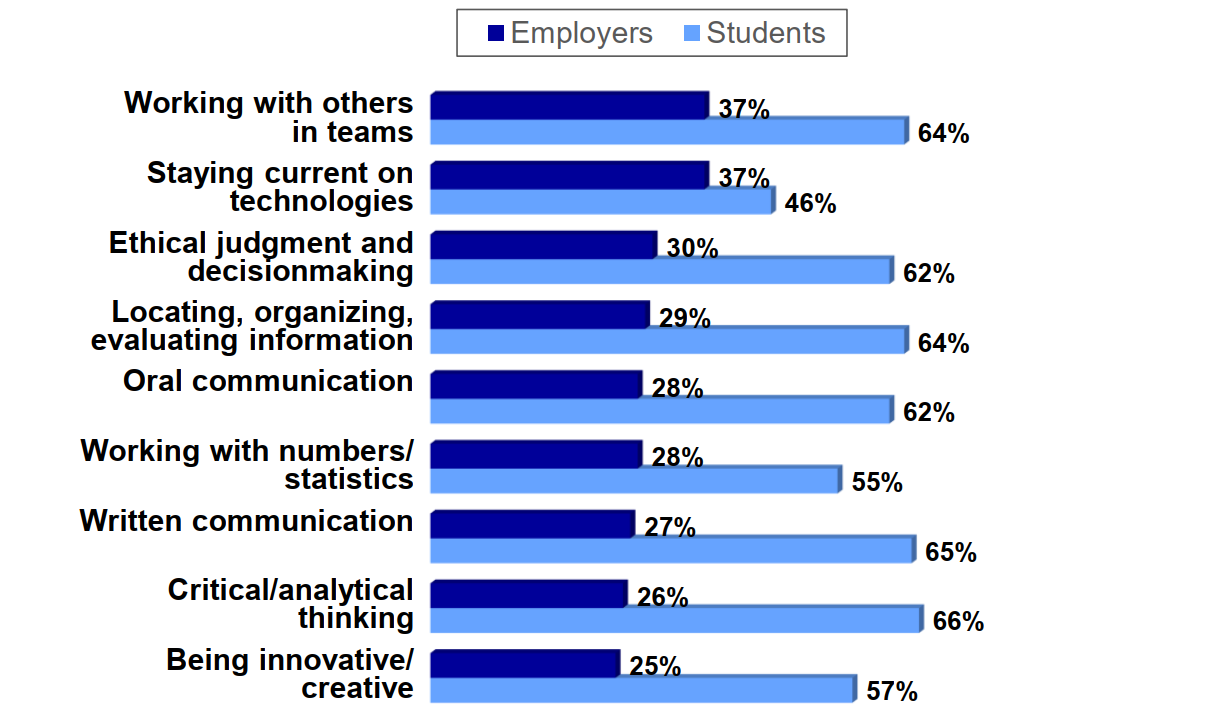
\includegraphics[width=250pt,height=147pt]{encuesta.png}
\caption{Porcentaje de habilidades blandas percibidas en el mercado laboral según perspectiva de los empleadores y de los estudiantes \cite{b9}.}
\label{fig:contexto_laboral}
\end{figure}

Casi la totalidad de los encuestados, tanto empleadores como estudiantes, creen que deberían tener un aprendizaje amplio y que se fomente el desarrollo de habilidades transversales a su especialidad, independientemente de su campo de estudio. Los empleadores además indicaron que los estudiantes deberían enfrentarse a experiencias que les permitan resolver conflictos con personas con opiniones diferentes a las propias \cite{b9} como parte de la currícula universitaria, en conjunto con el desarrollo de proyectos que fomenten su aprendizaje. Sin embargo, pese a esto, solo el 14\% de los empleadores encuestados opina que los estudiantes disponen de las habilidades y conocimientos necesarios para completar un proyecto aplicado que resulte significativo antes de su graduación. Por otro lado, un 53\% del total piensa que solo la mitad de ellos se encuentran preparados en este aspecto \cite{b9}.



\subsection{Situación percibida en el ámbito académico}
\label{scrivauto:14}

La situación laboral en términos de habilidades blandas es alarmante. Ante la carencia detectada de este tipo de cualidades y conocimientos, surge una necesidad concreta de fomentarlas en forma temprana, de estimular a los estudiantes para que puedan desarrollarlas y enfrentar con mayor preparación y competencia los desafíos del mundo profesional. Pero debido a que se tratan de habilidades que no se aprenden simplemente consultando un material de referencia, aún permanece el interrogante sobre cómo encarar esta labor.

Entre los meses de marzo y abril de 2020 se llevó a cabo una encuesta virtual a estudiantes de Dinamarca, Estonia, Grecia, Portugal y España con el propósito de estimar el contexto en Europa en carreras de ingeniería. La encuesta constó de dos partes: en la primera se evaluó la importancia percibida por los estudiantes sobre un listado propuesto de habilidades blandas; en la segunda, se les preguntó acerca de cuáles consideraban que eran los métodos de aprendizaje más propicios para fomentarlas \cite{b2}.

Se evaluaron un total de 44 habilidades blandas, agrupadas en cinco categorías, a saber:

\begin{itemize}
    \item Habilidades técnicas: que abarca cuestiones como la ética, consulta bibliográfica digital, nociones de salud y bienestar, entre otras.
    \item Habilidades metacognitivas: entre las que podemos mencionar el pensamiento crítico y la capacidad de evaluación de contenido de diversas fuentes.
    \item Habilidades intrapersonales: como ser la asertividad, la flexibilidad y la adaptabilidad.
    \item Habilidades interpersonales: trabajo en equipo, liderazgo, capacidad de escuchar a nuestros semejantes, interacción social y empatía.
    \item Habilidades de resolución de problemas: capacidad de aportar claridad a un conflicto, administración del tiempo y proyectos, implementación y evaluación de una solución potencial.
\end{itemize}

Para puntuarlas, se utilizó una escala del 1 al 5, donde 5 representa la máxima importancia percibida. Los resultados de esta encuesta pueden apreciarse en la figura \ref{fig:importancia_percibida}.


\begin{figure*}[htbp]
\centering
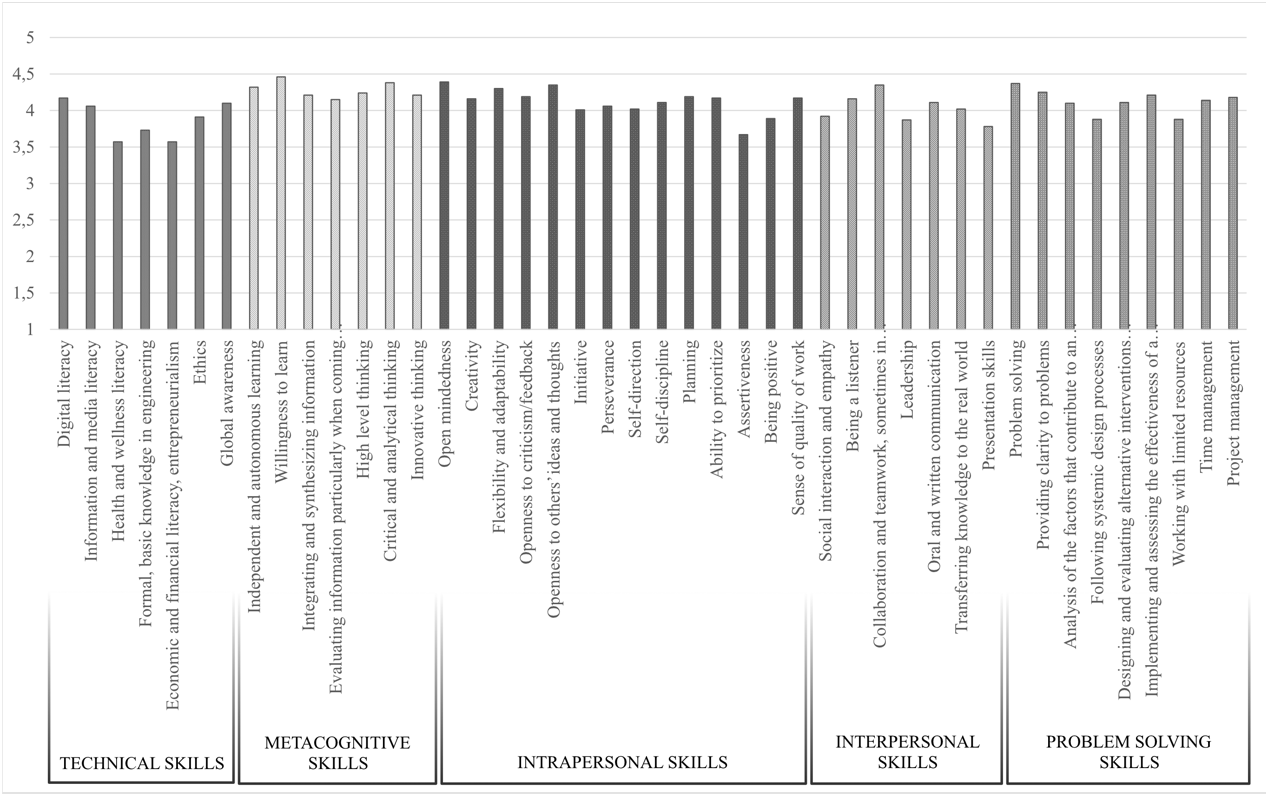
\includegraphics[width=450pt,height=282pt]{encuesta_soft_skills.png}
\caption{Importancia percibida por los estudiantes encuestados de las habilidades blandas expuestas \cite{b2}.}
\label{fig:importancia_percibida}
\end{figure*}

Es posible calcular la media ponderada para cada categoría y su desviación estándar con estos resultados. Mediante este proceso, se observa un hecho interesante que consiste en que los estudiantes consideran más importantes las habilidades metacognitivas, intrapersonales y de resolución de problemas que las técnicas en sí mismas \cite{b2}.

Para la segunda parte de la encuesta, acerca de la idoneidad de los métodos de enseñanza, se preguntó a los estudiantes si consideraban que la metodología actual era propicia para fomentar el desarrollo de las habilidades que consideraban importantes. Sorpresivamente, un 45\% se manifestó en desacuerdo y un 41\% permaneció indeciso con la respuesta \cite{b2}. Se les preguntó, en consecuencia, cuál consideraban que era el método idóneo para poder desarrollarlas. Las metodologías de aprendizaje posibles eran las siguientes:

\begin{itemize}
    \item Aprendizaje basado en problemas o proyectos. Se trata de un método que involucra actividades en las cuales se desafía a los estudiantes a resolver un problema o desarrollar un proyecto usando conocimientos de diversas especialidades. Esto permite simular la forma en que se utiliza el conocimiento en el mundo laboral. Algunos autores enfatizan el hecho de que hacer un proyecto que acompañe el programa analítico (situación muy frecuente en una gran cantidad de asignaturas) no es lo mismo que usar este modelo de aprendizaje. Mientras que el primero es solo una parte para reforzar un conocimiento, en el segundo el proyecto es principal y se convierte en el camino y la forma de aprender un conjunto de conocimientos.

    \item Aprendizaje basado en pensamiento. Pretende formar mejores pensadores focalizándose en fomentar el pensamiento crítico y creativo. Tiene un impacto completo en mejorar el bienestar profesional y personal, dado que involucra en su proceso la toma de decisiones, resolución de problemas concretos, evaluación de información, entre otros aspectos. 

    \item Pensamiento de diseño. Esta metodología permite introducir soluciones a problemas complejos y atender a las necesidades reales de los usuarios frente a las percibidas. Fomenta la empatía, ya que involucra un proceso de comprensión de las experiencias y los sentimientos de un grupo de usuarios ante un solución particular. También incorpora la lluvia de ideas (brainstorming) y el prototipado de soluciones potenciales con el fin de obtener retroalimentación.

    \item Aprendizaje basado en competencias.  Es una metodología que se centra en adquirir conocimiento de forma que los estudiantes puedan usarlo en situaciones reales.  Para esto se desarrollan una serie de actividades que fomentan determinadas competencias; cada una de ellas es un aprendizaje individual en sí mismo. Cada estudiante trabaja en una de ellas a la vez, antes de poder pasar a la siguiente.

    \item Aprendizaje cooperativo. Incentiva a los estudiantes a trabajar juntos para conseguir un objetivo específico. Se establecen actividades de manera que requieran interactuar y colaborar entre sí para completarlas.

    \item Ludificación (Gamification). Fomenta el aprendizaje mediante el uso de técnicas y dinámicas propias de los juegos y el entretenimiento (recompensas, reconocimiento, objetivos claros, sentido de grupo, etc.). 

    \item Aula invertida (Flipped Classroom). Es una técnica de aprendizaje mixto (blended) que pretende estimular el uso del tiempo fuera de clase para adquirir los conocimientos más elementales, con el fin de destinar las horas de clase para atender cuestiones más prácticas y cognitivas. Generalmente, el profesor provee un cierto material para leer antes de la clase. Los estudiantes revisan el material y usan el tiempo de clase para resolver preguntas, trabajar en ejercicios prácticos, etc. El profesor, entonces, juega el rol de mentor. Esta técnica permite un uso más eficiente del tiempo de clase y motiva a los estudiantes a tomar la responsabilidad de su propio aprendizaje.

\end{itemize}

La figura \ref{fig:met_preferidos} muestra un resumen de los resultados obtenidos. En ella, podemos apreciar que para carreras de Ingeniería y Economía el método más idóneo son el aprendizaje basado en proyectos y el basado en razonamiento.



\begin{figure}[htbp]
\centering
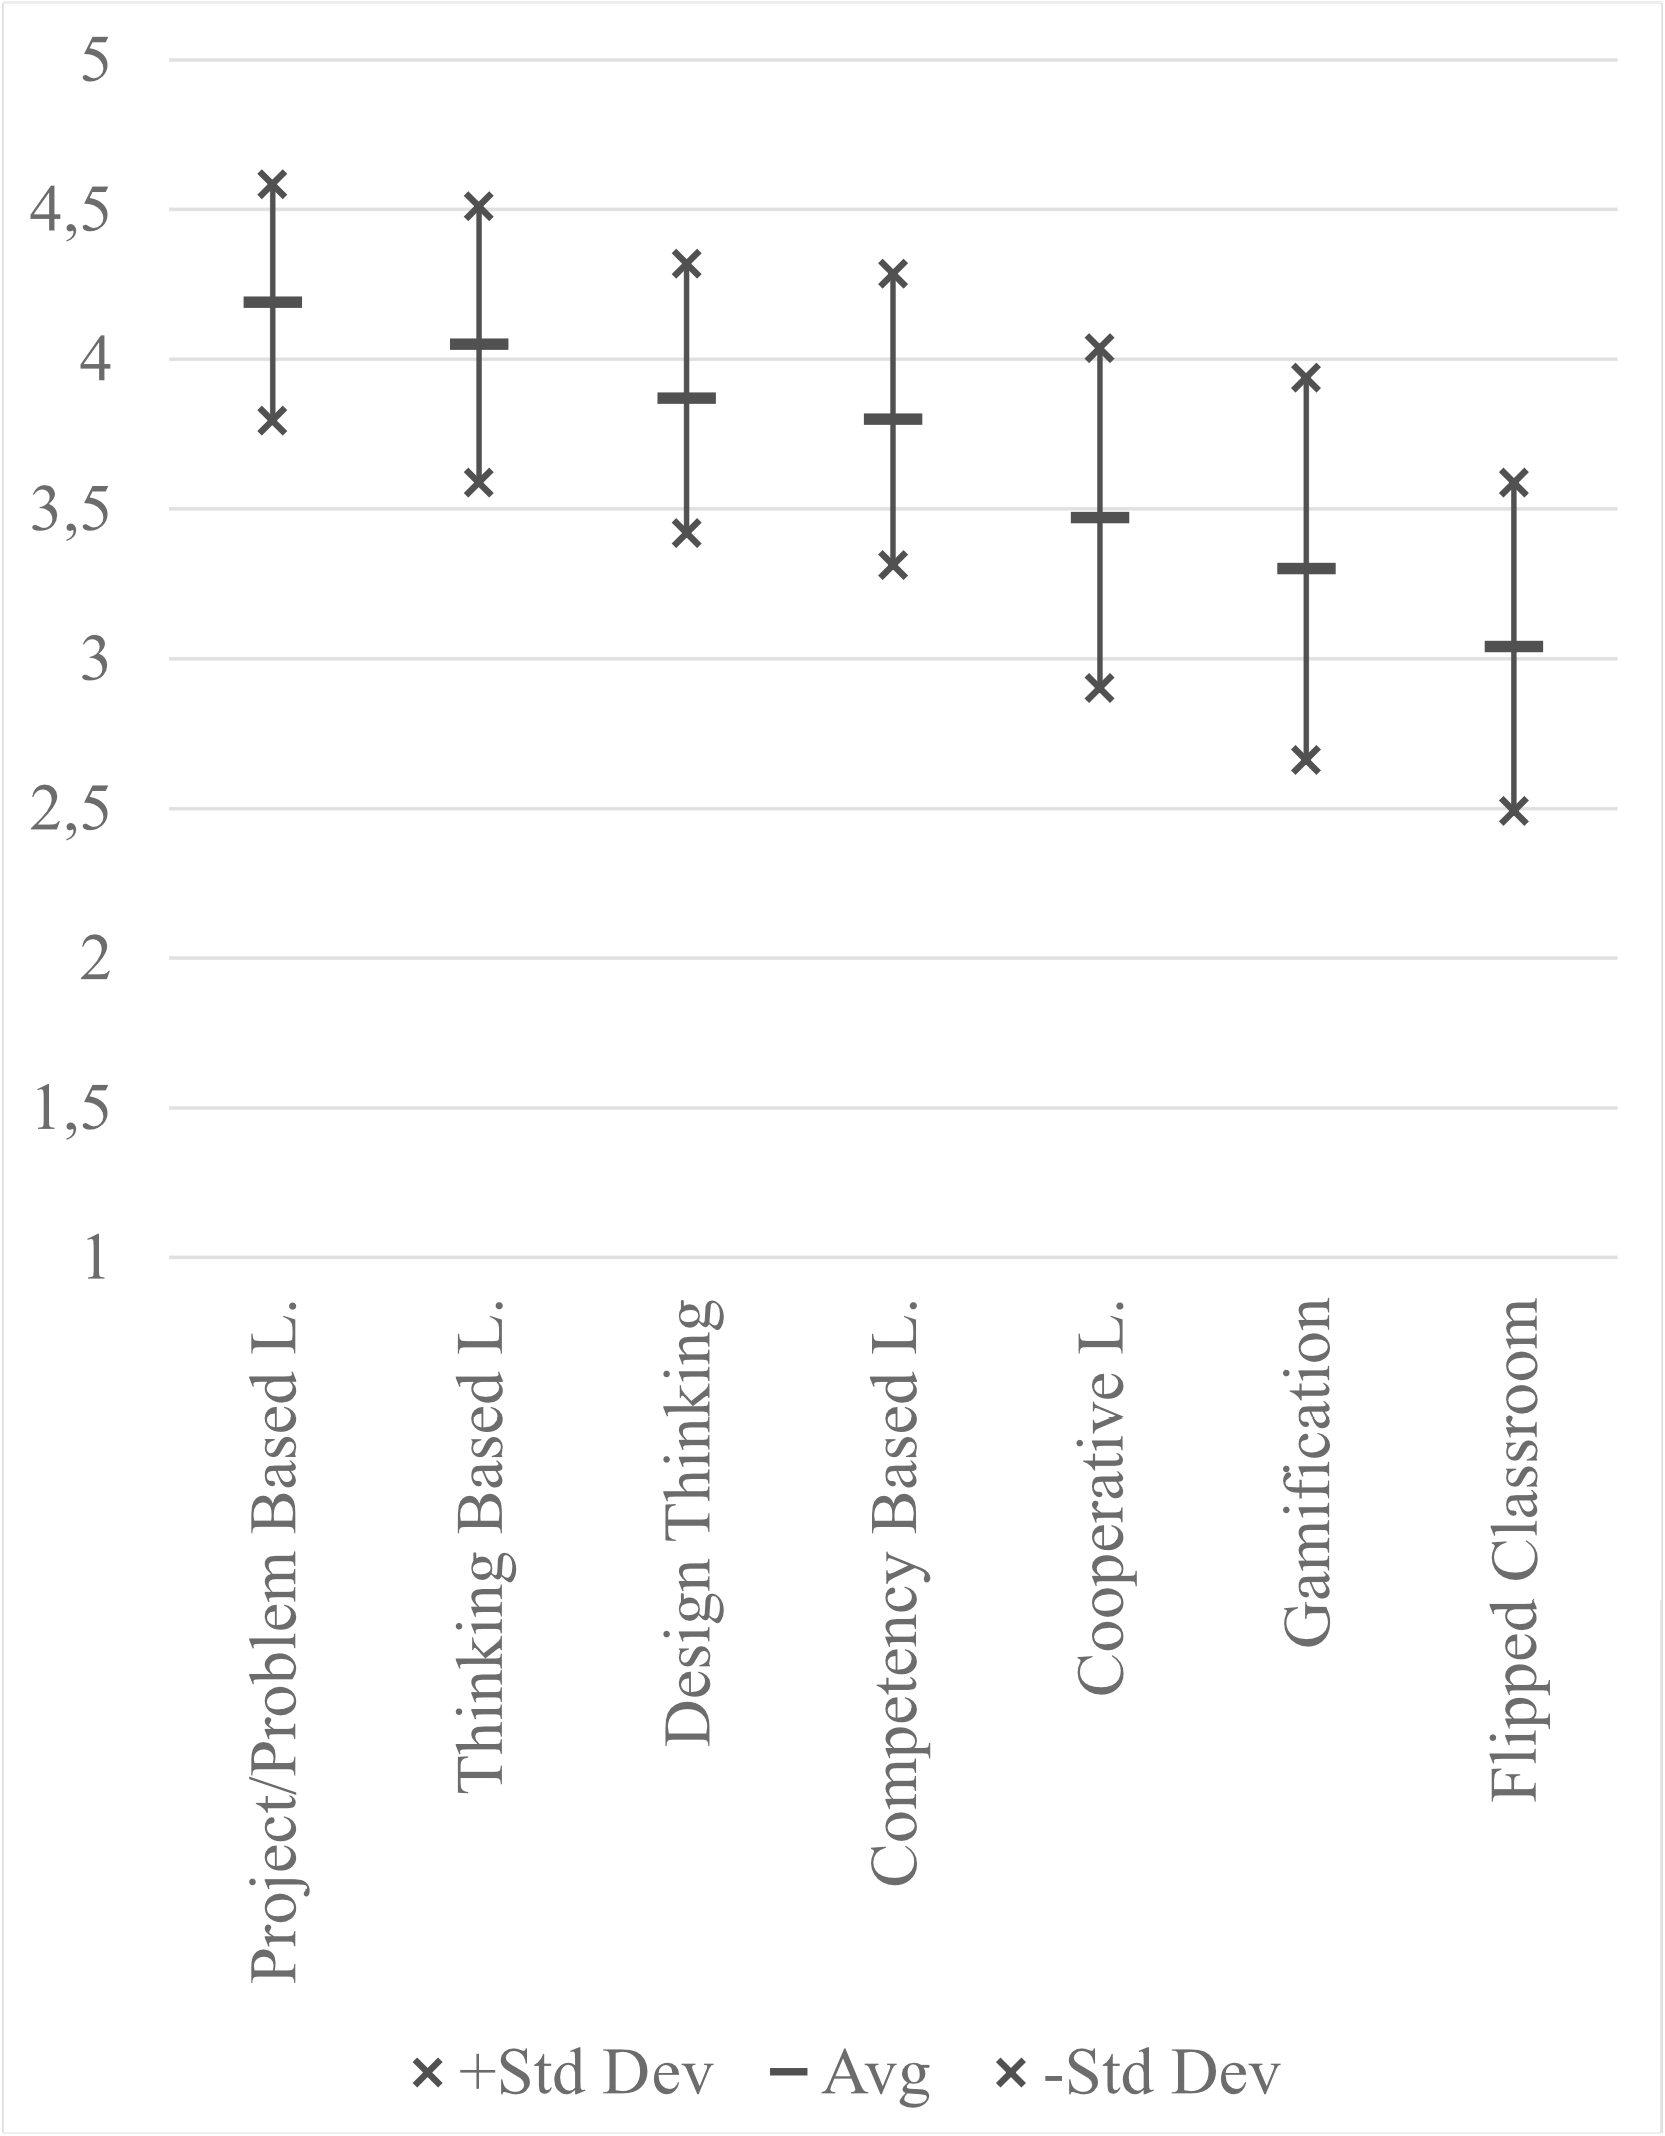
\includegraphics[width=250pt,height=321pt]{encuesta_learning.png}
\caption{Gráfica estadística resultante la encuesta a los estudiantes. Muestra los métodos de enseñanza más valorados por los encuestados.}
\label{fig:met_preferidos}
\end{figure}

\section{Debate y propuestas}
\label{scrivauto:15}

Tanto los empleadores como los propios estudiantes perciben una carencia en el sistema educativo, en términos de habilidades blandas. Mientras que los empleadores observan que los profesionales cada vez disponen menos de ellas. Por su parte, casi la mitad de los estudiantes no creen que las metodologías pedagógicas a las que se enfrentan sean las mejores para fomentarlas. Ambos hechos apuntan en la misma dirección: el sistema educativo presenta una carencia en lo que a habilidades blandas se refiere; es preciso efectuar un cambio para revertir esta situación.

Como se ha enunciado en la sección anterior, existen diversas metodologías de enseñanza, cada una de las cuales estimula un conjunto de habilidades específicas, siendo las siguientes las más valoradas por los estudiantes \cite{b2}.

\begin{itemize}
    \item Aprendizaje basado en problemas o proyectos (Problem/Project Based Learning)
    \item Aprendizaje basado en pensamiento (Thinking Based Learning)
\end{itemize}

Por otro lado, la motivación juega un papel fundamental en el rendimiento académico en el ámbito universitario \cite{b11}. Según el modelo de Pintrich (1994), la motivación académica depende de tres factores:

\begin{itemize}
    \item Contexto de la clase.
    \item Los sentimientos y creencias de los estudiantes sobre su propia motivación.
    \item Los comportamientos observables de los estudiantes.
\end{itemize}

A su vez, Pintrich explica que existen la motivación intrínseca y la extrínseca. La primera es propia de cada estudiante. La segunda, en cambio, es externa a ellos. Un estudiante desmotivado puede ocasionar que se preocupe más por aprobar con el mínimo esfuerzo que en aprender \cite{b11}. Así, con el fin de fomentar la propia motivación y atender las necesidades estudiantiles, se analizarán en detalle las metodologías de enseñanza mencionadas previamente y formas de implementarlas.


% Estas dos formas de aprendizaje son, según los estudiantes, las más óptimas para desarrollar sus propias habilidades blandas. Esto está sacado de B2.

% A modo de conocimiento e introducción, podría mencionar la existencia de los otros métodos, quizás{\ldots} Depende de cómo vaya armando el documento.


\subsection{Aprendizaje basado en problemas o proyectos}
\label{scrivauto:16}

Esta metodología de enseñanza se utiliza en el campo de la medicina desde la década de 1960 \cite{b12}. Sin embargo, pese a que existe hace años, en algunas áreas aún no se implementa. Tal es el caso de las carreras de ingeniería y afines donde aún se suelen utilizar clases demostrativas con ejercicios complementarios y, eventualmente, un proyecto que acompañe el programa de la asignatura. Esa metodología clásica, denominada por algunos autores como ``chalk and talk``, si bien tiene beneficios en la incorporación de habilidades duras, no favorece la incorporación de las blandas.

A menudo se suele confundir el aprendizaje basado en proyectos o problemas (en ambos casos, PBL) con simplemente acompañar la enseñanza en pizarrón o el material de estudio con algún caso práctico o desarrollo. Sin embargo, PBL pretende utilizar un proyecto o problema ya no como un complemento, sino como medio de enseñanza en sí mismo para incorporar una serie de conocimientos técnicos y blandos al mismo tiempo.

A lo largo del tiempo hubo varios intentos por aplicar PBL en estudios de ingeniería. Un ejemplo de esto es la carrera de Ingeniería Química de la McMaster University, descripto en varias publicaciones \cite{b12}, que utilizó PBL en dos cursos de sus cursos: uno a nivel de segundo año y otro en uno de diseño de proyectos. Para cumplir con este propósito, se gestionó un ``Programa de resolución de problemas`` conformado por cuatro talleres repartidos en cursos de varios niveles. Estos talleres ayudan al estudiante a adquirir habilidades interpersonales y a trabajar en equipo, permitiéndoles encarar la resolución de un proyecto en grupos, sin necesitar de un tutor asignado. En realidad, analizando esta cuestión, puede apreciarse que la solución provista por la universidad de McMaster incluye varias metodologías distintas y que el aprendizaje basado en proyectos es solo una de sus componentes \cite{b12}.

En 2013, la Universidad Politécnica de Madrid, en España, lanzó una iniciativa para brindar soporte a los profesores acerca del uso de PBL, dado que muchos de ellos no estaban familiarizados con la metodología \cite{b2}. Fundó además el proyecto ``Core Competencies in Engineering. Proposal of a Model for the UPM`` que fue una de las partes de uno mayor de innovación educativa, que tuvo lugar entre 2010-2017 \cite{b10}. Entre las habilidades seleccionadas para este programa encontramos el trabajo en equipo, comunicación oral y escrita, creatividad, respeto por el medio ambiente, liderazgo y resolución de problemas. La meta detrás de esta iniciativa fue que los estudiantes pudieran adquirir y desarrollar cada uno de estos aspectos, además de los conocimientos requeridos para la especialidad.

El procedimiento que siguieron para emprender esta metodología está basado en los enunciados de Pólya \cite{b10}.

\begin{itemize}
    \item Comprensión del problema, esto implica leer la consigna y analizarla de varias formas. Reconocer los temas conocidos y los que falta por conocer.
    \item Planificar la solución, involucra analizar los datos para obtener un bosquejo de una solución.
    \item Implementar el plan, pudiendo requerirse modificaciones en el proceso.
    \item Evaluar el resultado y el procedimiento utilizado, esencial para mejorar y fomentar el correcto aprendizaje.
\end{itemize}

Siguiendo estos lineamientos, se desarrolló un conjunto de reglas genéricas para orientar al alumno sobre los principales aspectos y en qué orden encararlos para resolver el problema. Los problemas propuestos difieren mucho según la asignatura y el nivel de estudios, por lo que se dividió la iniciativa en cuatro niveles, cada uno con un procedimiento propio y con reglas diferentes \cite{b10}. El punto del orden en que se analizan los aspectos principales del problema no es un dato menor. En PBL, el orden en que se aprenden los conocimientos está parcialmente definido por los estudiantes, lo que podría dar lugar a que algunos temas se pasen por alto. Mientras que en algunas especialidades es posible este paradigma y aprender lo restante en otro momento, en carreras como ingeniería, matemáticas y física, muchos conceptos 	se deben aprender en un orden específico	. La carencia de ciertos conocimientos puede ser difícil de corregir para el estudiante \cite{b12}.

\subsection{Aprendizaje basado en pensamiento}
\label{scrivauto:17}

El aprendizaje basado en pensamiento (TBL, por sus siglas en inglés) es una metodología activa de enseñanza que se centra en que los estudiantes aprendan a pensar, a razonar y a tomar decisiones, mientras adquieren los conceptos del temario de estudios \cite{b13}. Es un escenario propicio para ganar experiencia contrastando fuentes de información o formulando hipótesis. Los profesores actúan de guías, presentando una serie de cuestiones que los incentiva a pensar por sí mismos de forma analítica y crítica.

Esta metodología presenta una serie de ventajas destacables, entres las cuales podemos mencionar:

\begin{itemize}
    \item Es una metodología activa. Esto implica un rol diferente al tradicional tanto para el cuerpo docente como para el alumnado, quienes deben construir el conocimiento guiados por el profesor a cargo. 
    \item Según el campo de aplicación, es capaz de estimular habilidades blandas como la reflexión, la ética profesional, el trabajo en equipo, la toma de decisiones y el pensamiento analítico.
    \item Puede ser complementario a otras metodologías. Así, puede combinarse con el aprendizaje basado en proyectos, el trabajo colaborativo y la pedagogía inversa.
\end{itemize}

 Para su implementación, es necesario enseñar con antelación a los estudiantes cómo ejercer un pensamiento crítico, proveerle una serie de criterios mínimos a considerar justificando su importancia. Luego, cuando ya están preparados, pueden por ejemplo trabajar en grupos para tratar un tema en concreto. En esta metodología, es frecuente valerse de una serie de recursos como mapas de razonamiento y tablas para organizar información, o preguntas específicas relacionadas al propósito de la clase.

En \cite{b14} se cita un ejemplo del aprendizaje basado en pensamiento aplicado a la resolución de una consigna de impacto ambiental y fuentes energéticas. Se propone a los estudiantes un escenario en que forman parte de un comité y se les solicita que informen cuál será la fuente de energía más dominante en los próximos 25 años. Junto a esta consigna, se plantea un mapa de razonamiento que establece los puntos claves de la toma de decisión, a saber:

\begin{itemize}
    \item ¿Por qué es necesaria la decisión?
    \item ¿Cuáles son nuestras opciones?
    \item ¿Cuáles son las consecuencias de esas opciones?
    \item ¿Qué tan importantes son esas consecuencias?
    \item ¿Cuál es la mejor opción en vistas de esas consecuencias?
\end{itemize}

De esta forma, los estudiantes tienen un punto de partida concreto y definido para empezar el análisis. Como podemos suponer a partir de este ejemplo, no solamente están aprendiendo acerca de las fuentes energéticas, energías renovables y no renovables, sino que también adquieren todas las cuestiones laterales a lo estrictamente técnico. En otras palabras, todo lo que necesitan saber para ser capaces de elaborar una decisión por sí mismos o en trabajo colaborativo.

\section{Conclusiones}
\label{scrivauto:18}

En este artículo se planteó un panorama completo acerca de qué son las habilidades blandas. Si bien no existe un consenso claro acerca de cómo clasificarlas, se plantearon dos posibilidades, ambas útiles según el grado de análisis que se necesite efectuar en ellas.

En base a los resultados de las encuestas, es posible observar que el sistema académico presenta una carencia en este campo. Se deben buscar formas de promover y fomentar las habilidades blandas desde cada institución. Para atender este punto, se propusieron dos posibles metodologías de enseñanza: el aprendizaje basado en proyectos o problemas, y el basado en pensamiento. Pese a sus diferencias, ambos son complementarios y fomenta cada uno un conjunto de habilidades diferente.

Se analizó la aplicación de PBL en las áreas de ingeniería y afines. Se concluye que es posible, pero puede requerir otras metodologías anexas o talleres que la acompañen. Finalmente, se observa que la aplicación de PBL está limitada en estas carreras por el orden en que se deben aprender los conocimientos técnicos para asegurar un aprendizaje consistente.

En cuanto a TBL, se concluye que es una metodología orientada a forjar el razonamiento crítico en los estudiantes, planteándoles situaciones en que deben tomarse decisiones, analizar el mundo en un contexto dado, buscar las razones de un fenómeno y analizar posibles solución a un problema dado y su impacto.

\begin{thebibliography}{00}

\bibitem{b1} C. Stewart, A. Wall, y S. Marciniec, ``Mixed Signals: Do College Graduates Have the Soft Skills That Employers Want?'', Competition Forum. 14. 276-281, 2016.
% Habla de la situación de las empresas.

\bibitem{b2} M. Caeiro-Rodríguez et al., ``Teaching Soft Skills in Engineering Education: An European Perspective'', in IEEE Access, vol. 9, pp. 29222-29242, 2021, doi: 10.1109/ACCESS.2021.3059516.
% Acá menciona muchas formas de aprendizaje. Puede estar bueno para atender la sección métodos de aprendizaje

\bibitem{b3} B. Schulz, ``The Importance of Soft Skills: Education beyond academic knowledge'', Journal of Language and Communication. 2. 10.1016/0006-3207(93)90452-7. 2008.
% 

\bibitem{b4} G. A. Meeks, ``Critical Soft Skills to Achieve Success in the Workplace'',  Walden Dissertations and Doctoral Studies, 2017.
% De acá saco definiciones de hard y soft skills

\bibitem{b5} D. Hutagalung, A. Sopa, M. Asbari, Y. Cahyono, S. Maesaroh, G. Chidir, y D. S. Winanti, ``Influence soft skills, hard skills and organization learning on teacher’s performance through inovation capability as mediator'', J Crit Rev, 7, 54-66, ISSN- 2394-5125, 2020.
% De acá saco definiciones de hard skills

\bibitem{b6} D. Beard, D. Schwieger, K. Surendran, ``Integrating Soft Skills Assessment through University, College, and Programmatic Efforts at an AACSB Accredited Institution,'' Journal of Information Systems Education, Vol. 19(2), 229-240, 2008
% 

\bibitem{b7} E. A. Gnatyshina, N. V. Uvarina, A. Savchenkov, N. A. Pakhtusova, y N. Y. Korneeva, ``Soft skills in young people in regions'', Laplage em Revista, vol. 7, nº Extra-A, p. p.449-455, mayo 2021.
% Acá habla de qué permiten las habilidades blandas respecto a lo profesional
% Propone agruparlas en cuatro categorías o ejes fundamentales.
% Tiene un estudio muy interesante, se encuestó a varias personas para sacar conclusiones acerca de las soft skills.

\bibitem{b8} ``Self-Presentation''. [Online] Accedido el:  de junio de 2021. Disponible en: https://psychology.iresearchnet.com/papers/self-presentation/
% De acá saqué la definición de self-presentation. Está asociado a la gestión de impresiones ante una audiencia: https://en.wikipedia.org/wiki/Impression_management

\bibitem{b9} Hart Research Associates, ``Falling short? College learning and career success. Association of American Colleges and Universities'', 2015.
% Esta es una encuesta de dónde se sacó parte de la info para redactar el b1. Parece muy útil.

\bibitem{b10}  A. Mendez, M. Florensa, C. Molleda, A. Alcazar, C. Fernandez, y J. B. D. Ramiro, ``Development of a method of assessment of the problem solving competence at the technical university of madrid'', Int. J. Eng. Educ., vol. 30, no. 6, pp. 1749--1758, 2014.
% Acá propone una forma de aplicar PBL en carreras de ingeniería. Es uno de los papers en que se basó b2.

\bibitem{b11} A. Anaya-Durand, y C. Anaya-Huertas, ``¿Motivar para aprobar o para aprender? Estrategias de motivación del aprendizaje para los estudiantes'', Tecnología, ciencia, educación, 25(1), 5-14, 2010.
% Acá habla de la motivación y el modelo de Pintrich. No tengo acceso al material original, así que tengo que citar esta fuente abierta.

\bibitem{b12} J. E. Mills, y D. F. Treagust, ``Engineering education---Is problem-based or project-based learning the answer. Australasian journal of engineering education'', 3(2), 2-16, 2003.
% Esto habla de las dificultades de aplicar PBL en carreras de ingeniería.

\bibitem{b13} Grupo SM, ``Thinking-Based Learning''. Accedido el: 8 de junio de 2021.  [Online] Disponible en: https://www.grupo-sm.com/sites/sm-espana/files/resources/Imagenes/MKT/Recursos-did%C3%A1cticos/TBL-Thinking-Based-Learning.pdf
% Acá propone una forma de aplicar TBL. Está interesante.

\bibitem{b14} R. J. Swartz, ``Thinking-Based Learning. Making the Most of What we Have Learned About Teaching in the Regular Classroom to Bring Out the Best in Our Students'', Educational Leadership, 65(5), 2008.
% Acá propone una forma de aplicar TBL. Está interesante.


\end{thebibliography}
\vspace{12pt}

\end{document}